\glsresetall
\chapter{Alleviation of Data Scarcity for Radar-Based ECG Recovery} \label{ch:RFcardi}
This chapter focuses on the data scarcity in the training of \gls{dnn} for radar-based ECG recovery. In the previous research, most studies either develop advanced signal processing methods to improve SNR~\cite{liu2024diversity,zhang2023overview} or leverage various deep learning frameworks to realize accurate ECG recovery~\cite{zhao2024airecg,zhang2024radarODE-MTL}. However, the method for reducing dependence on data quantity is rarely investigated for radar-based ECG recovery, and all the deep-learning-based ECG recovery models are trained in a supervised manner~\cite{chen2022contactless,zhao2024airecg,li2024radarnet}. In this chapter, a transfer learning framework is proposed following \gls{ssl} paradigm to extract cardio-related information from the radar signal without ECG ground truth based on the intrinsic sparsity of cardiac features, and only a few synchronous radar-ECG pairs are required to fine-tune the pre-trained model for the ECG recovery. In addition, a data augmentation method is designed to increase the diversity of input samples while the augmented spectrogram is still faithful to the original ground truth vital sign.

\section{Introduction}
The trials on the radar-based ECG recovery can be categorized into two paradigms. The first paradigm only performs the extraction of high-resolution cardiac mechanical activities to produce quasi-ECG signals, omitting the morphological ECG features while maintaining certain fine-grained features. For example, the mostly adopted quasi-ECG signal only preserves R and T peaks and can be realized by signal decomposition~\cite{dong2024robust} or state estimation~\cite{ji2022rbhhm,xia2021radar}. In contrast, the second paradigm aims to reconstruct the ECG waveform as measured by clinical apparatus, because the doctor and ECG analysis toolbox all rely on the shape of ECG to make diagnosis~\cite{makowski2021neurokit2}. However, decoupling the ECG signal from the measured radar signal requires establishing an extremely complex model from the perspective of electrophysiology (i.e., excitation-contraction coupling~\cite{swift2021stop}), and the existing research can only leverage deep learning methods to learning such domain transformation from the dataset containing numerous radar/ECG pairs~\cite{chen2022contactless,wu2023contactless,wang2023ecg,zhang2024radarODE}.
 
Similar to all the research fields involved with deep learning, radar-based ECG recovery also asks for numerous radar signals to train the deep learning model with synchronous ECG ground truths~\cite{li2024radarnet,zhang2024radarODE-MTL,chu2024vessel}. However, data scarcity is an inevitable issue, because radar system requires expertise in configuration setting and signal pre-processing and the ECG collection requires cumbersome procedures, causing difficulties for the deployment in new scenarios with limited data. 

In the literature, data augmentation and SSL are two popular methods to alleviate data scarcity, but there is no existing work that applies them in radar-based ECG recovery. Firstly, most augmentation techniques are designed for classification problems, and the inputs (signal or image) can be safely masked/recombined/flipped/stretched without changing the ground truth (labeled class). However, the aforementioned techniques are not applicable to the regression-based vital sign reconstruction (e.g. radar-based ECG recovery), because the changes on the input cannot be directly applied on the ground truth ECG, e.g., the real ECG peaks have a similar width, therefore randomly stretching the ECG signals is unfaithful to the biological facts~\cite{swift2021stop}. Secondly, SSL, as another popular technique for reducing dependence on data quantity, is rarely investigated for radar-based ECG recovery, and all the deep-learning-based ECG recovery models are trained in a supervised manner with the large dataset containing $3-32$ hours of synchronous radar-ECG pairs~\cite{chen2022contactless,zhao2024airecg,li2024radarnet}. 

\begin{figure}[tb]
        \centering
        \subfloat[]{\label{fig:spec_trad}\includegraphics[width=0.4\columnwidth]{sst_aug_trad.pdf}}\vspace{0.01\columnwidth}
        \subfloat[]{\label{fig:bad}\includegraphics[width=0.4\columnwidth]{bad_result.pdf}} \\
        \subfloat[]{\label{fig:spec_hp}\includegraphics[width=0.4\columnwidth]{sst_aug_hp.pdf}}\vspace{0.01\columnwidth}
        \subfloat[]{\label{fig:good}\includegraphics[width=0.4\columnwidth]{good_result.pdf}}
        \caption{Illustration of Horcrux: (a) Traditional augmentation with zero mask; (b) Missed detected heartbeat (HB) and distorted ECG recovery; (c) Horcrux with time consistency preserved; (d) Ideal cardiac monitoring with high fidelity.}
        \label{fig:hp_compare}
\end{figure}

Based on the discussion above, the contributions of this study can be listed as: 
\begin{itemize}
\item A data augmentation method called Horcrux is designed for extracting cardiac features from radar by preserving the intrinsic time consistency hidden in the input radar spectrogram to restrict the potential distribution shift as illustrated in Figure~\ref{fig:hp_compare}, expanding the diversity of the limited training dataset without distorting the key features.
\item A transfer learning framework RFcardi is proposed following an SSL paradigm to effectively learn the latent representations from radar signals by leveraging an appropriate pre-text task. Accordingly, this work further designates the \gls{ssr} as the pre-text task, assisting the RFcardi to learn essential representations for the later ECG recovery.
\item The experimental results illustrate that the proposed Horcrux outperforms the existing augmentation methods in both classification and regression tasks (i.e., heartbeat detection and ECG recovery). In addition, the pre-trained RFcardi framework can be easily adapted to realize radar-based ECG recovery with a small amount of synchronous radar-ECG measurements for fine-tuning. 
\end{itemize}

The rest of the chapter is organized as follows. Section~\ref{sec:data_augm} and~\ref{sec:tf_design} elaborates the proposed Horcrux and RFcardi framework, with the experimental results shown in Section~\ref{sec:exp_cp6} and~\ref{sec:exp_cp6_1}. The final conclusion is shown in Section~\ref{sec:conclusion_cp7}.

\section{Data Augmentation for Radar Spectrogram}\label{sec:data_augm}
\subsection{Overview} 
The overview of the proposed Horcrux is based on the signal model in (\ref{equ:vib_long}) and is depicted in Figure~\ref{fig:HP_pipline} with two parallel modules:
\begin{itemize}
\item The \gls{hp} decomposition module decomposes the original radar signal into the harmonic and percussive components, with the former referring to the stable component along certain frequency bands on a spectrogram and the latter representing the transient component with a pulsatile nature occurring at certain time indices, as shown in the red boxes in Figure~\ref{fig:HP_pipline}.
\item The \gls{dtm} module aims to figure out the most characteristic vibration based on the signal template in (\ref{equ:vib_long}) and output the corresponding time indices $T_1, T_2$ and central frequencies $f_1,f_2$ (omit $k$ for simplicity), with the comparison between the raw and synthetic radar signal shown in Figure~\ref{fig:HP_pipline}.
\end{itemize}
The traditional augmentation methods either cannot be directly applied to the ground truth data or could potentially erase the crucial part for prediction (especially for heartbeat detection), as shown in Figure~\subref*{fig:spec_trad}. Therefore, Horcrux only masks the spectrogram of harmonic component and preserves the percussive feature, as shown in Figure~\subref*{fig:spec_hp}. In addition, by deliberately masking the related part based on $T_1, T_2, f_1, f_2$, it is expected that the well-trained deep learning model will concentrate more on the regions that help cardiac feature extraction instead of being distracted by the noises spread on the spectrogram.

\begin{figure}[tb] 
    \centering 
    \includegraphics[width=0.99\columnwidth]{HP_pipline.pdf}
    \caption{Pipeline of Horcrux with two branches: (a) Harmonic and percussive (H$\&$P) components decomposition; (b) Dynamic template matching.} 
    \label{fig:HP_pipline} 
\end{figure}

\subsection{Harmonic and Percussive Components Decomposition} 
Signal decomposition is widely used in signal processing to identify components with different features and help the downstream algorithm extract target information e.g., \gls{ica} decomposes the signal from different sources based on statistical independence, and \gls{emd} decomposes the signal based on the oscillatory modes with different time scales~\cite{chen2022contactless}. Considering the nature of the cardiac activities, the radar signal reflected from the chest region reveals two characteristics on the spectrogram: (a) the stable components along certain frequency bands that represent either the heart rate frequency (near $1$Hz) or the center frequency of the prominent vibrations ($10-25$ Hz)~\cite{zhang2024radarODE-MTL}; (b) the transient components simply indicates the pulsatile heartbeats with large energy. In this research, these two components are named harmonic and percussive components (features) as highlighted in the red boxes in Figure~\ref{fig:HP_pipline}.

The decomposition process is based on the spectrogram $\mathcal{Y}(m, n)$ obtained using any time-frequency representation tools such as synchrosqueezed wavelet transform~\cite{zhang2024radarODE-MTL}, with $m$ and $n$ indicating the time frame index and frequency bin index, respectively. Then, the median filter $\mathcal{F}(\cdot)$ is applied along the time axis of $\mathcal{Y}(m,n)$ to get the harmonic-enhanced spectrogram as:
\begin{equation}
Y_h(m, n)=\mathcal{F}(\mathcal{Y}(m, n), k_h)
\end{equation}
where the median filter replaces the middle value within a window length $k_h$ by the median value in this window and is widely used in image and signal processing. 

Similarly, the percussion-enhanced spectrogram can be obtained using a median filter with window length $k_p$ along the frequency axis as:
\begin{equation}
Y_p(m, n)=\mathcal{F}(\mathcal{Y}(m, n), k_p)
\end{equation}

Then, a soft mask based on the Wiener filter is suggested in~\cite{fitzgerald2010harmonic} to adaptively suppress the unwanted components, and the Wiener masks $M_h$ and $M_p$ for isolating harmonic and percussive component from the original spectrogram are calculated as:
\begin{equation}
\begin{aligned}
M_h(m,n)&=\frac{Y_h(m,n)}{Y_h(m,n)+Y_p(m,n)}\\
M_p(m,n)&=\frac{Y_p(m,n)}{Y_h(m,n)+Y_p(m,n)}
\end{aligned}
\end{equation}

Lastly, the harmonic spectrogram $\mathcal{Y}_h(m, n)$ and percussive spectrogram $\mathcal{Y}_p(m, n)$ can be obtained as:
\begin{equation}
\begin{aligned}
\mathcal{Y}_h(m, n)=M_h(m, n) \otimes \mathcal{Y}(m, n)\\
\mathcal{Y}_p(m, n)=M_p(m, n) \otimes \mathcal{Y}(m, n)
\end{aligned}
\end{equation}
with $\otimes$ representing element-wise multiplication, and the resultant spectrograms are shown in Figure~\ref{fig:HP_pipline} with the corresponding features enhanced. In addition, it can be observed that certain percussive features are still revealed on the harmonic component and vice versa, because the soft Wiener mask can not totally eliminate the other component with much larger energy on the spectrogram. In addition, the Horcrux augmentation does not require a complete separation of H\&P component, H\&P decomposition module is to preserve the percussive features, therefore it is acceptable

\subsection{Dynamic Template Matching (DTM)}
The DTM module is designed to figure out the regions in the time- and frequency-domain that are closely related to the prominent vibrations, encouraging the deep learning model to focus on these regions for capturing crucial information. According to the literature~\cite{zhang2024radarODE-MTL}, the time indices $T_1,T_2$ of the prominent vibrations can be identified by the deep learning model based on their central frequencies $f_1,f_2$, and Horcrux proposes to dynamically obtain these four parameters for each input segment as a template matching problem to find the optimal parameter set:
\begin{equation}\label{equ:opt_equ}
\begin{aligned}
{\theta}^*=\underset{{\theta=\{T_1,T_2,f_1,f_2\}}}{\arg \min } &\left\|y(t)-\tilde{d}(t, \theta)\right\|_2  \\
\text{Subject to: } &T_2-T_1<\tau
\end{aligned} 
\end{equation}
where $y(t)$ is the segment from dataset and $\tilde{d}(t,\theta)$ represents the signal synthesized from (\ref{equ:vib_long}) with the parameter set ${\theta}$. The constraint represents that $T_2$ always follows $T_1$ within a distance $\tau$, because the identified vibrations should belong to the same cardiac cycle and the time interval between aortic valve opening ($T_1$) and closure ($T_2$) should be less than $\tau$ sec~\cite{swift2021stop}. 

To simplify the optimization, only one cardiac cycle is considered for one segment, and only the key parameters (i.e., $\theta=\{T_1,T_2,f_1, f_2\}$) are left to be determined with initial values shown in Table~\ref{tab:sm_param}, while the values of other parameters are empirically assigned as shown in Table~\ref{tab:sm_param}. In addition, the optimization problem in (\ref{equ:opt_equ}) is solved by sequential least squares programming (SLSQP) to yield optimal parameter set $\theta^*$ that indicates the time indices and central frequencies of the prominent vibrations as shown as the synthetic signal in Figure~\ref{fig:HP_pipline}.

\begin{table}[tb]
\centering
\caption{Parameters for signal model}
    \begin{tabular}{cc?cc?cc?cc}
    \toprule
    \textbf{Par.} & \textbf{Value} & \textbf{Par.} & \textbf{Value} & \textbf{Par.} & \textbf{Value} & \textbf{Par.} & \textbf{Value} \\
    \toprule
    $T_1$ & $0.4$  & $T_2$  & $0.85$ &$f_1$ & $10$  & $f_2$  & $23$  \\
    \midrule
    $a_1$ & $0.5$  & $a_2$  & $0.1$ & $b_1$ & $0.05$  & $b_2$  & $0.03$ \\
    \bottomrule
    \end{tabular}%
\label{tab:sm_param}
\end{table}%
\subsection{Augmented Spectrogram Generation}
The last step of Horcrux is to randomly select one vibration from $v_1,v_2$ and mask the corresponding regions on the harmonic spectrogram based on $\theta^*$ with the width of $w_t$ or $w_f$ for time or frequency domain. The applied zero mask alters the data distribution of the original spectrogram to enhance the diversity of the limited dataset, and the deep learning model will concentrate more on the masked regions selected by the DTM module with informative features for cardiac activities, as shown in Figure~\ref{fig:HP_pipline}.

Lastly, the harmonic spectrogram with zero mask is added with the percussive spectrogram yielded from H$\&$P decomposition module to provide necessary information that preserves time consistency in the final Horcrux augmentation spectrogram as shown in Figure~\ref{fig:HP_pipline}. In addition, the added percussive spectrogram restricts the shift of data distribution brought by zero masks, and the augmented spectrogram still shares a similar representation with the normal spectrogram that is used in the evaluation or test stage of deep neural work training.


\section{Transfer Learning Framework Design}\label{sec:tf_design}
\subsection{Deep Learning Model Design}
In the previously designed data deep learning model~\cite{zhang2024radarODE-MTL}, the radar signals with high-SNR should be convert to spectrograms, providing extra frequency-domain information to assist model training. The deep learning model adopts the popular backbone-decoder structure as designed in~\cite{zhang2024radarODE-MTL}:
\begin{itemize}
  \item The backbone leverages ResNet~\cite{he2020resnet} framework with deformable 2D convolution layer~\cite{dai2017deformable} to efficiently extract cardiac features from image-like spectrogram inputs.
  \item The decoder is based on 1D convolutional neural network (CNN) to generate corresponding signals either for the pre-text task or ECG signal recovery. 
\end{itemize}

\subsection{Pre-text Task Training and Fine-tuning}
Inspired by other signal-based research~\cite{zhang2025umimo,chen2024tfpred}, transfer learning is a promising paradigm to learn the latent representation from unlabeled radar signal to capture basic cardiac features in an SSL manner, reducing the requirement of cumbersome ECG collection. Then, only a small amount of synchronous radar-ECG pairs is required to fine-tune the pre-trained model to realize the ECG recovery for new scenarios. The proposed RFcardi framework adopts high-SNR radar signals as inputs to pre-train the backbone with \gls{ssr} as the pre-text task. Then, the same backbone will used for the fine-tuning stage so that the latent representations learned in the pre-trained model can be seemly transferred for the ECG recovery task, as shown in Figure~\ref{fig:rfcardi}.

\begin{figure}[tb] 
    \centering 
    \includegraphics[width=0.95\columnwidth]{RFcardi.pdf}
    \caption{Illustration of RFcardi with pre-text training and fine-tuning stages.} 
    \label{fig:rfcardi} 
\end{figure}


The efficient SSL requires an appropriate design of the pre-text task to help the deep learning model capture essential features that assist ECG recovery, and the pre-text task used for SSL should reveal certain inherent features in the radar-monitored vital sign. Two major features used for traditional heart rate estimation are periodicity and sparsity~\cite{zhang2023overview}. In this work, the duration of each segment is $4$ sec and may not reveal strong periodicity. Therefore, SSR will be used as the pre-text task in RFcardi and is defined as:
\begin{equation}
h=\Phi x+n
\end{equation}
where $h$ is the high-SNR radar signal, $\Phi$ means the observation matrix, $x$ is the sparse representation for heartbeats and $n$ represents the residual noise. The traditional SSR task can be seemly converted to a system identification problem by viewing $\Phi$ as a multi-channel adaptive filter, and the estimation of the filter coefficient is the same as training a CNN-based neural network (i.e., training CNN kernels)~\cite{ha2020contactless}.

In this case, the SSR task is realized by using the aforementioned CNN-based backbone-decoder structure with the loss function:
\begin{equation}\label{equ:sparse}
\mathcal{L} = \|x -x^{\prime} \|_2 + \underbrace{\lambda_s\frac{\|x\|_1 / \| x\|_2-1}{\sqrt{m}-1}}_{\text{sparse penalty}}
\end{equation}
where $m$ is the length of the signal, $x$ is the output the from deep learning model, $x^{\prime}$ is the sparse ground truth with values for the radar peaks maintained (1st vibration in Figure~\subref*{fig:target_org}) while other values are set to $0$. The sparse penalty has a range of $[0,\lambda_s)$ with a smaller value indicating better sparsity~\cite{hoyer2004non}.

After pre-training based on SSR, the parameters of backbone will be retained with a new decoder connected (same structure as for pre-text task training), and a few radar-ECG pairs are used for fine-tuning the pre-trained RFcardi model using MSE as the loss function.


\section{Experimental Results for Horcrux}\label{sec:exp_cp6}
\subsubsection{Evaluation Metrics}
For the evaluation of the proposed data augmentation method Horcrux, the performance of the ECG recovery and heartbeat detection are evaluated from the following perspectives:
\begin{itemize}
\item \textbf{Root mean square error (RMSE)}: RMSE describes the morphological fidelity of the recovered ECG signal and is sensitive to the peak deviation.
\item \textbf{Pearson-correlation coefficient (PCC)}: PCC also reveals morphological fidelity but is sensitive to the general shape of the recovered ECG signal.
\item \textbf{Heartbeat error (H. E.)}: Heartbeat error simply shows the absolute timing error of the detected heartbeat with the ground truth.
\item \textbf{Missed detection rate (MDR)}: MDR is a metric to assess the performance of deep learning model against noises by calculating the percentage of the missed detected heartbeats, because the strong noise (e.g., body movement) or low SNR scenarios may drown the subtle cardiac features and cause missed detection.
\end{itemize}
In addition, to comprehensively evaluate the overall performance of each method, $\Delta m\%$ is adopted as in many multi-task learning studies to assess the performance based on multiple metrics as:
\begin{equation}\label{equ:mdr1}
\Delta m\%=\frac{1}{n} \sum_{i=1}^{n} S_{i, j} \frac{M_{m,i}-M_{b, i}}{M_{b, i}} \times 100\%
\end{equation}
where $n$ is the number of metrics, $M_{m,i}$ means the performance of a method $m$ measured by metric $j$, $M_{b,i}$ means the performance of the baseline, and $S_{i, j}=1\text{ or }0$ if lower or higher values are better for the current metric (indicated by $\downarrow\text{ or }\uparrow$).

\subsection{Evaluation for DTM}
The DTM module aims to figure out the most prominent vibrations for a certain cardiac cycle within a $4$-sec input segment, and the illustration of the performance under different radar signal qualities (SNR) is shown in Figure~\ref{fig:temp_match}. It is worth noticing that the proposed DTM module not only identifies the prominent vibrations under good signal quality (e.g., Figure~\subref*{fig:eg_0} and~\subref*{fig:eg_2}), but could tolerant the low-SNR scenarios with certain constant noise drowning the characteristic peaks (e.g., Figure~\subref*{fig:eg_4} and~\subref*{fig:eg_5}). 

\begin{figure}[tbp]
        \centering
        \subfloat[]{\label{fig:eg_0}\includegraphics[width=0.4\columnwidth]{synthetic_signal_3.pdf}}
        \subfloat[]{\label{fig:eg_1}\includegraphics[width=0.4\columnwidth]{synthetic_signal_0.pdf}}\\
        \subfloat[]{\label{fig:eg_2}\includegraphics[width=0.4\columnwidth]{synthetic_signal_2.pdf}}
        \subfloat[]{\label{fig:eg_3}\includegraphics[width=0.4\columnwidth]{synthetic_signal_1.pdf}}\\
        \subfloat[]{\label{fig:eg_4}\includegraphics[width=0.4\columnwidth]{synthetic_signal_5.pdf}}
        \subfloat[]{\label{fig:eg_5}\includegraphics[width=0.4\columnwidth]{synthetic_signal_6.pdf}}
        \caption{Identified vibrations using DTM for radar signals with various qualities (illustrated in normalized amplitude).}
        \label{fig:temp_match}
\end{figure}

In addition, the DTM module could successfully identify $87\%$ and $53\%$ of the first and the second prominent vibrations ($v_1$ and $v_2$) within the absolute tolerance of $0.15$s~\cite{chen2022contactless}, ensuring a precise mask applied on the spectrogram in Horcrux. The specific impacts of the DTM module on the final ECG recovery quality will be evaluated in the later ablation study section, and the wrong detection in DTM will not degrade the overall performance of Horcrux because applying a random mask also contributes to the radar-based ECG recovery.

\subsection{Evaluation for Horcrux}
\subsubsection{Comparison with State-of-the-art Methods}
The performance of the proposed Horcrux is shown in Table~\ref{tab:res} in terms of RMSE, PCC, H. E. and MDR, with the comparison among the state-of-the-art augmentation methods for regressions tasks by mixing up the input and ground truth within homogeneous samples~\cite{hwang2024rc,schneider2024anchor,yao2022c}. In addition, the Horcrux is implemented on the dataset with different proportions to evaluate the impact of masks on the change of data distributions and model performance as shown in Table~\ref{tab:res}.

From Table~\ref{tab:res}, Horcrux achieves the best result when applying on $20\%$ of the dataset with an overall improvement of $16.20\%$ and outperforms all the existing augmentation methods, because the mix-up-based methods enhance the diversity of the dataset in sacrificing the time consistency inside one cardiac cycle. Therefore, the mix-up-based methods show less improvement or even degradation in RMSE and PCC, while Horcrux preserves the percussive component to maintain the time consistency inside the spectrogram. However, the masks applied on the spectrogram still change the data representation, and the overuse of Horcrux may cause the drift in the learned data representation or distribution, causing the degradation starting from the ECG recovery, as indicated by the bad RMSE and PCC in Table~\ref{tab:res} for Horcrux ($25\%$ and $30\%$).


\begin{table}[tbp]
  \centering
  \caption{Comparison of different augmentation methods}
  \begin{tabular}{lcccc|c}
  \toprule
  Methods & \makecell[c]{RMSE \\ (mV) } $\downarrow$ & PCC $\uparrow$ & \makecell[c]{H. E. \\ (ms) } $\downarrow$ & MDR $\downarrow$ &  $\Delta m\%$\\
  \midrule
  \textbf{Baseline} & 0.096 & 82.65\% & 8.82 & 6.73\% & 0.0\% \\
  \midrule
  C-Mixup~\cite{yao2022c} & \underline{0.088} & 82.25\% & 7.55 & 6.14\% & 7.80\% \\
  ADA~\cite{schneider2024anchor} & 0.097 & 81.28\% & 7.20 & 6.69\% & 4.12\% \\
  RC-Mixup~\cite{hwang2024rc} & 0.089 & 83.36\% & 7.72 & 5.79\% & 8.69\% \\
  \midrule
  \textbf{Horcrux} ($10\%$) & 0.096 & 82.24\% & 6.89 & 6.67\% & 5.63\% \\
  \textbf{Horcrux} ($15\%$) & 0.087 & \underline{84.75\%}& 6.96 & \textbf{5.19\%} & \underline{14.02\%} \\
  \textbf{Horcrux} ($20\%$) & \textbf{0.086} & \textbf{85.41\%} & \underline{6.21} & \underline{5.30\%} & \textbf{16.20\%} \\
  \textbf{Horcrux} ($25\%$) & 0.092 & 81.99\% & \textbf{6.16} & 6.36\% & 9.81\% \\
  \textbf{Horcrux} ($30\%$) & 0.094 & 80.18\% & 6.55 & 6.59\% & 6.78\% \\
  \bottomrule
  \multicolumn{6}{r}{The best/second best results are indicated by \textbf{Bold}/\underline{underline}.} \\
  \end{tabular}
  \label{tab:res}
\end{table}

\subsubsection{Ablation Study}
The improved performance achieved by Horcrux comes from two aspects, i.e., H$\&$P decomposition and DTM module, and an ablation study is performed to specify the contributions as shown in Table~\ref{tab:aug-res}. Firstly, the original spectrogram is used as inputs with masks applied in the time or frequency domain randomly or based on the DTM module. It is worth noticing that simply applying random masks on the original set could achieve an improvement of $8.42\%$, and masking the frequency domain ($7.04\%$) contributes more than masking the time domain ($4.28\%$), because zero mask will cover all the useful information and affects heartbeat detection. This phenomenon can also be verified by precisely masking the prominent vibrations based on DTM, causing the heavy degradation with negative $\Delta m\%$ as shown in Table~\ref{tab:aug-res}.

In addition, the H$\&$P decomposition itself also improves the cardiac features extraction with an improvement of $8.57\%$, because the percussive and harmonic features are both enhanced after adding them up. Afterward, the random mask could further improve the performance to $9.86\%$, while the DTM-based mask achieves the largest improvement of $16.20\%$. It is also worth noticing that only masking the time domain ($13.18\%$) achieves a better result than covering the frequency domain ($10.69\%$), because the H$\&$P decomposition preserves the percussive information, and the heartbeat is still detectable even after masking the prominent vibrations precisely.

\begin{table}[tbp]
  \centering
  \caption{Ablation study for Horcrux}
  \resizebox{\textwidth}{!}{
  \begin{tabular}{c|cc|cc|cccc|c}
  \toprule
  \multirow{3}*{\textbf{Input}} & \multicolumn{2}{c|}{\textbf{{Mask Type}}} & \multicolumn{2}{c|}{\textbf{{Selected Domain}}} & \multicolumn{4}{c|}{\textbf{\makecell[c]{Evaluation Metrics}}} & \multirow{3}*{$\Delta m\% $} \\
   & Random & DTM & Time & Frequency & \makecell[c]{RMSE \\ (mV) } $\downarrow$ & PCC $\uparrow$ & \makecell[c]{H. E. \\ (ms) } $\downarrow$ & MDR $\downarrow$ \\
  \midrule
  \multirow{7}*{\makecell[c]{Original \\ Spectrogram \\ (without Horcrux)}} &-&-&-&-& 0.096 & 82.65\% & 8.82 & 6.73\% & 0.0\% \\
    &\ding{52}&         &\ding{52}&          & 0.089 & 82.86\% & 7.14 & 7.38\% & 4.28\% \\
    &\ding{52}&         &         &\ding{52} & 0.088 & 83.53\% & 7.80 & 6.27\% & 7.04\% \\
    &\ding{52}&         &\ding{52}&\ding{52} & 0.087 & 83.03\% & 7.26 & 6.25\% & 8.42\% \\
    &         &\ding{52}&\ding{52}&          & 0.089 & 83.71\% & 9.53 & 6.34\% & -1.13\% \\
    &         &\ding{52}&         &\ding{52} & 0.099 & 80.00\% & 8.03 & 7.01\% & -0.24\% \\
    &         &\ding{52}&\ding{52}&\ding{52} & 0.098 & 81.19\% & 7.88 & 7.95\% & -2.41\% \\
  \midrule
  \multirow{7}*{\makecell[c]{H$\&$P \\ Spectrogram \\ (with Horcrux)}} &-&-&-&-& 0.091 & 83.73\% & 7.45 & 5.92\% & 8.57\% \\
    &\ding{52}&         &\ding{52}&          & \underline{0.084} & 85.40\% & \underline{6.90} & 6.71\% & 9.48\% \\
    &\ding{52}&         &         &\ding{52} & 0.086 & 84.03\% & 8.26 & \underline{5.35\%} & 9.86\% \\
    &\ding{52}&         &\ding{52}&\ding{52} & 0.085 & 84.89\% & 7.22 & 5.74\% & 11.80\% \\
    &         &\ding{52}&\ding{52}&          & \textbf{0.083} & 84.94\% & 7.04 & 5.72\% & \underline{13.18\%} \\
    &         &\ding{52}&         &\ding{52} & 0.085 & \textbf{87.20\%} & 7.96 & 5.66\% & 10.69\% \\
    &         &\ding{52}&\ding{52}&\ding{52} & 0.086 & \underline{85.41\%} & \textbf{6.21} & \textbf{5.30\%} & \textbf{16.20\%} \\
  \bottomrule
  \multicolumn{10}{r}{The best/second best results are indicated by \textbf{Bold}/\underline{underline}.} \\
  \end{tabular}
  }
  \label{tab:aug-res}
\end{table}

\begin{figure}[tbp] 
    \centering 
    \includegraphics[width=0.6\columnwidth]{performance.pdf}
    \caption{Performance of using different scales of the dataset.} 
    \label{fig:perfor} 
\end{figure}
\subsubsection{Performance under Different Dataset Scale}
As a data augmentation technique, Horcrux is tested with different scales of dataset with the overall performance $\Delta m\%$ shown in Figure~\ref{fig:perfor}. It is notable that the degradation of the performance is not in a linear relationship with the input data scale, showing an obvious tipping point after axing the input data to $80\%$ without augmentation. After applying Horcrux, the performance is boosted using the same scale of input data as already proved by the previous ablation study. In addition, the deep learning model with Horcrux reveals a mild degradation with reduced input data, and the occurrence of the tipping point is also postponed to $70\%$ as shown in Figure~\ref{fig:perfor}, because the faithful alteration of the data representation could improve the generalization of deep learning model and alleviate the risk of overfitting.

\section{Experimental Results for RFcardi}\label{sec:exp_cp6_1}
For the evaluation of the proposed transfer learning framework RFcardi, the experimental results are illustrated for the SSL stage and fine-tuning stage, respectively.
\subsection{Evaluations and Ablation Studies of SSL}
The SSR task is crucial in the proposed transfer learning framework to provide latent representation that assists the further ECG pattern recovery, reducing the demand for radar-ECG pairs in the fine-tuning stage. The results of SSL are shown in Table~\ref{tab:ssr} in terms of MSE and sparsity to illustrate the former and latter part (without $\lambda_s$) in the loss function (\ref{equ:sparse}) for SSL training.

The experiment is repeated for different dataset scales with the ablation study on the use of sparse penalty, and the results indicate that both MSE and sparsity decrease with the reducing training data as shown in Table~\ref{tab:ssr}. Training with $100\%$ or $80\%$ dataset could achieve convergence and realize a successful SSR with similar MSE ($0.0091, 0.0082$) or ($0.0096, 0.0085$). However, the performance of SSR degrades heavily when further decreasing the training data without the constraint of sparse penalty, because the SSR results might fluctuate, as shown in Figure~\subref*{fig:ssr_bad}. In contrast, introducing the sparse penalty could suppress the fluctuation and force the deep learning model to focus only on the dominant peaks of the input radar signals, as shown in Figure~\subref*{fig:ssr_good}. Therefore, the training with sparse penalty loss still achieves good results with an MSE of $0.0092$ and $0.0098$ by using $60\%$ and $40\%$ of the dataset, while the model cannot be well-trained without sparse penalty by using $40\%$ dataset as shown in Table~\ref{tab:ssr} and Figure~\subref*{fig:ssr_bad}.
\begin{table}[tb]
\centering
\caption{Performance of SSL with ablation study}
    \begin{tabular}{c|cc?cc}
    \toprule
    {Methods} & \makecell[c]{MSE \\ ($\times 10^2$)} $\downarrow$ & Sparsity $\downarrow$ & \makecell[c]{MSE \\($\times 10^2$)} $\downarrow$ & Sparsity $\downarrow$ \\
    \midrule
    & \multicolumn{2}{c?}{\textbf{$\mathbf{100\%}$ Dataset}} & \multicolumn{2}{c}{\textbf{$\mathbf{80\%}$ Dataset}}  \\
    \midrule
    SSL w/o sp$^*$ & $0.91$ & $0.36$  & $0.96$ & $0.41$ \\
    SSL with sp    & $0.82$ & $0.20$  & $0.85$ & $0.22$ \\
    \midrule
    & \multicolumn{2}{c?}{\textbf{$\mathbf{60\%}$ Dataset}} & \multicolumn{2}{c}{\textbf{$\mathbf{40\%}$ Dataset}} \\
    \midrule
    SSL w/o sp & $1.43$ & $0.44$  & \multicolumn{2}{c}{Failed}\\
    SSL with sp    & $0.92$  & $0.26$  & $0.98$  & $0.31$\\
    \bottomrule
    \multicolumn{5}{l}{$^*$sp for sparse penalty}
    \end{tabular}%
\label{tab:ssr}
\end{table}%

\begin{figure}[tb]
  \centering
  \subfloat[]{\label{fig:ssr_bad}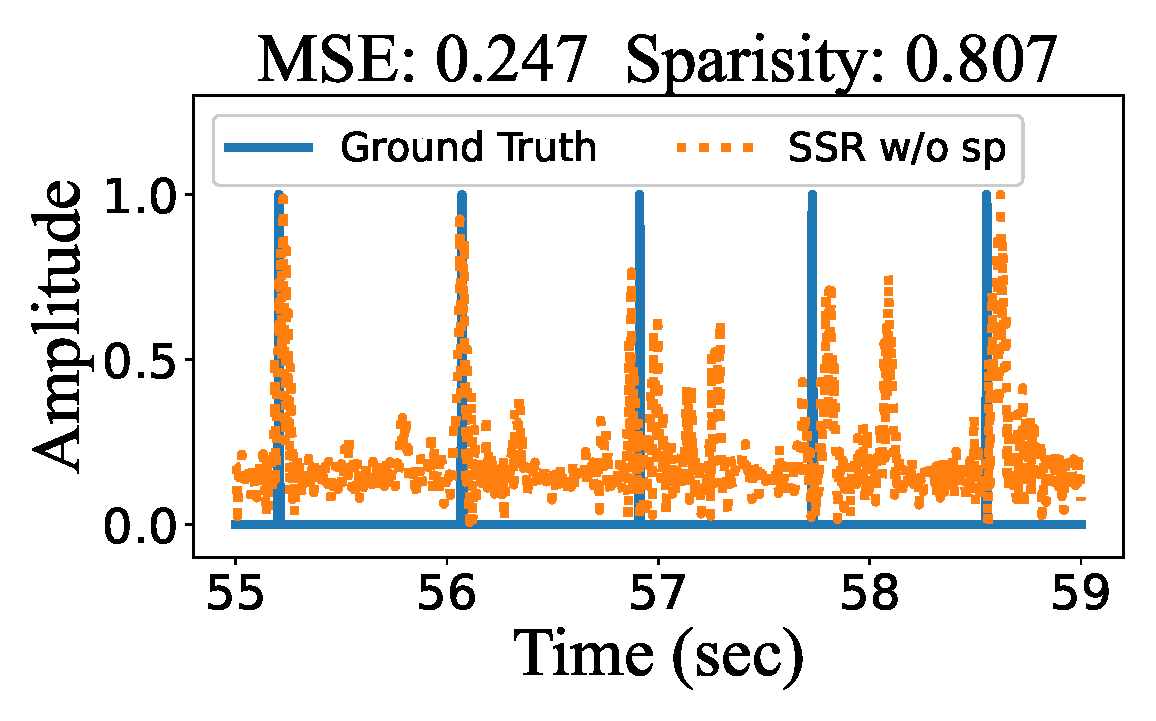
\includegraphics[width=0.4\columnwidth]{ssr_bad.eps}}
  \subfloat[]{\label{fig:ssr_good}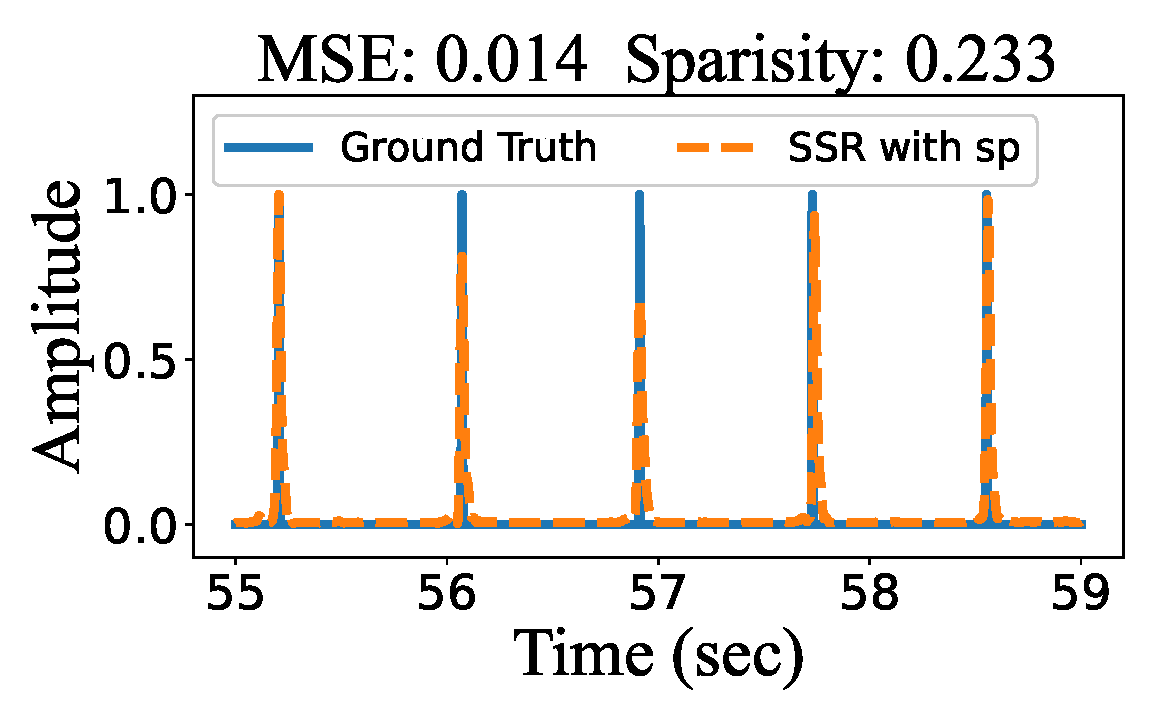
\includegraphics[width=0.4\columnwidth]{ssr_good.eps}}
  \caption{Results of SSR: (a) Failed SSR due to lack of data and sparse penalty; (b) Ideal SSR result with good MSE and sparsity.}
  \label{fig:ssr_res}
\end{figure}
\subsection{Evaluations of Fine-tuning Results}
The fine-tuning is based on the model pre-trained by $100\%$ dataset with or without sparse penalty, and the experiment is repeated for different percentages of labeled data (i.e., radar signal with ECG ground truth). In addition, the same deep-learning model will be trained in a supervised manner by using the same amount of labeled data as the reference for transfer-learning ECG recovery. At last, an overall improvement will be provided by calculating the percentage of improvement across all four metrics to provide straightforward evaluations for different methods, as shown in Table~\ref{tab:ecg_few_shot}.

\begin{table}[tb]
\centering
\caption{Performance of ECG recovery using different percentages of labeled data}
\resizebox{\textwidth}{!}{
    \begin{tabular}{c |cccc|c?cccc|c}
    \toprule
    {Methods} & \makecell[c]{MSE\\($\times 10^{-2}$)} $\downarrow$ & PCC $\uparrow$ & \makecell[c]{Peak Error \\ (ms)} $\downarrow$ & MDR $\downarrow$ & Overall $\uparrow$ & \makecell[c]{MSE\\($\times 10^{-2}$)} $\downarrow$ & PCC $\uparrow$ & \makecell[c]{Peak Error \\ (ms)} $\downarrow$ & MDR $\downarrow$  & Overall $\uparrow$\\
    \toprule
    &\multicolumn{5}{c?}{\textbf{$\mathbf{100\%}$ Labeled}} & \multicolumn{5}{c}{\textbf{$\mathbf{80\%}$ Labeled}} \\ 
    \midrule
    Supervised & ${0.80}$ & ${85.47\%}$ & ${7.61}$ & ${6.85\%}$ & $0.00\%$ & $0.84$ & $84.60\%$ & $8.90$ & $8.04\%$ & $-10.09\%$ \\
    {TF w/o sp$^*$} & $0.81$ & $85.35\%$ & $8.46$ & $5.51\%$ & $1.75\%$ & $0.82$ & $86.36\%$ & $8.35$ & $7.02\%$ & $-3.42\%$ \\
    {TF with sp} & $0.80$ & $85.51\%$ & $8.40$ & $5.14\%$ & $3.66\%$ & $0.81$ & $84.29\%$ & $8.31$ & $7.14\%$ & $-4.02\%$ \\
    \midrule
       & \multicolumn{5}{c?}{\textbf{$\mathbf{60\%}$ Labeled}} & \multicolumn{5}{c}{\textbf{$\mathbf{40\%}$ Labeled}} \\ 
    \midrule
    Supervised & $0.93$ & ${79.91\%}$ & ${10.65}$ & ${8.93\%}$ & $-23.27\%$ & $0.98$ & $75.89\%$& $11.15$ & $12.15\%$ & $-39.4\%$\\
    {TF w/o sp} & $0.85$ & $83.74\%$ & $8.84$ & $8.65\%$ & $-12.68\%$ & $0.97$ & $76.56\%$ & $10.87$ & $10.99\%$ & $-34.05\%$ \\
    {TF with sp} & $0.86 $& $84.92\%$ & $8.58$ & $7.72\%$ & $-8.71\%$ & $0.93$ & $78.72\%$ & $8.70$ & $9.02\%$ & $-17.54\%$ \\
    \bottomrule
    \multicolumn{5}{l}{$^*$TF for transfer learning and sp for sparse penalty}
    \end{tabular}%
    }
\label{tab:ecg_few_shot}
\end{table}%

The fine-tuning with $100\%$ labeled data provides very similar performance in morphological accuracy with the MSE and PCC around $0.0080$ and $85.47\%$. It is worth noticing that the peak error and MDR are slightly improved, because the pre-text task SSR for pre-training is equivalent to identifying the peak position of the radar signal, and the learned representations can be seemly transferred to improve the accuracy of the recovered ECG R peaks, contributing to the overall improvement for transfer learning ($3.66\%$ and $1.75\%$).

Reducing $20\%$ of labeled data causes a $10\%$ overall degradation as shown in Table~\ref{tab:ecg_few_shot}, and the decline of peak error and MDR is more than MSE and PCC. The reason is that ECG morphological patterns for different cardiac cycles are similar and can be well-learned from $80\%$ labeled data with good MSE and PCC ($0.0084$ and $84.60\%$), while the location of each ECG piece is random and can be distorted by noises, requiring more training data for convergence.

The supervised training with $60\%$ labeled data cannot ensure a good morphological and peak accuracy and the overall degradation is $23.37\%$, with the PCC drop below $80\%$ as shown in Table~\ref{tab:ecg_few_shot}. In contrast, the pre-trained model still provided good results with mild degradations of $8.71\%$ and $12.68\%$. It is noticed that the effectiveness of sparse penalty in the SSL stage also affects the fine-tuning stage, because both peak error and MDR for transfer learning with spare penalty are better than those without sparse penalty, causing a large gap in the overall improvement compared with the previous training with $100\%$ and $80\%$ dataset.

Lastly, the deep learning model can barely learn from $40\%$ labeled dataset and yield a bad morphological and peak accuracy for supervised learning. In addition, examples of the recovered ECG for transfer learning with or without sparse penalty are shown in Figure~\ref{fig:fs_res}, and it is clear that the deep learning model struggles to learn both morphological and peak features from limited data if the pre-text task is not well-trained without sparse penalty, while Figure~\subref*{fig:fs_good} shows the good recovery because the pre-trained model transfer the learned representations from radar inputs to ECG recovery.
\begin{figure}[tb]
  \centering
  \subfloat[]{\label{fig:fs_bad}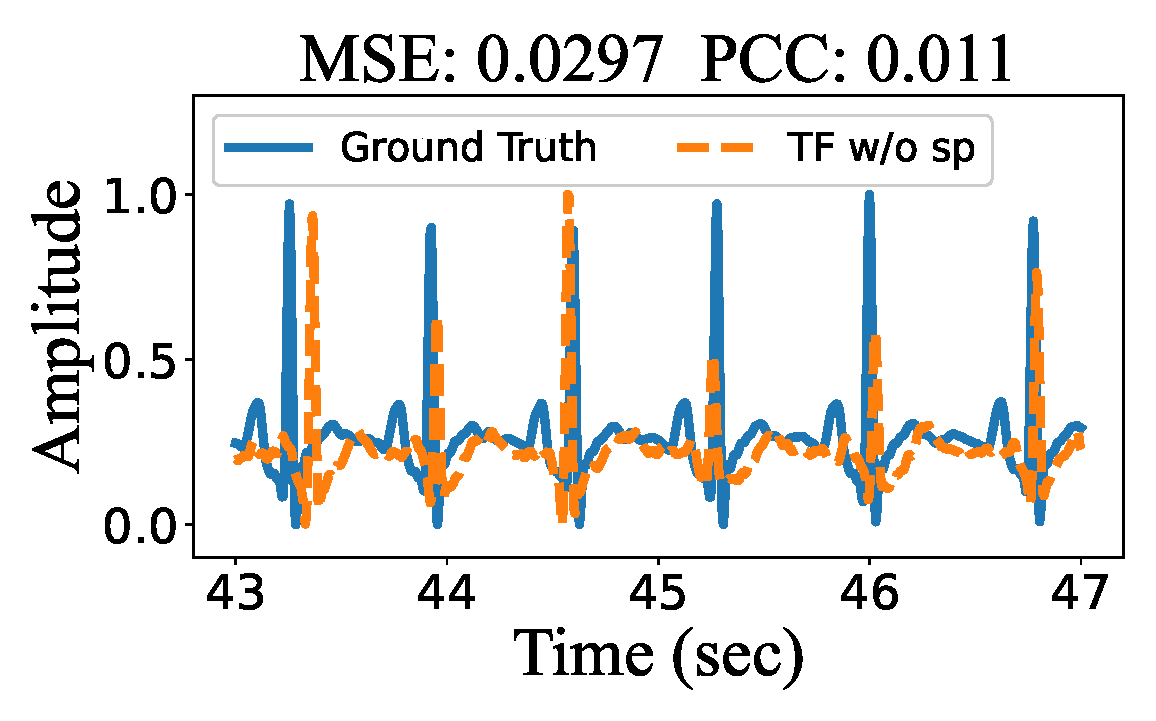
\includegraphics[width=0.4\columnwidth]{fs_bad.eps}}
  \subfloat[]{\label{fig:fs_good}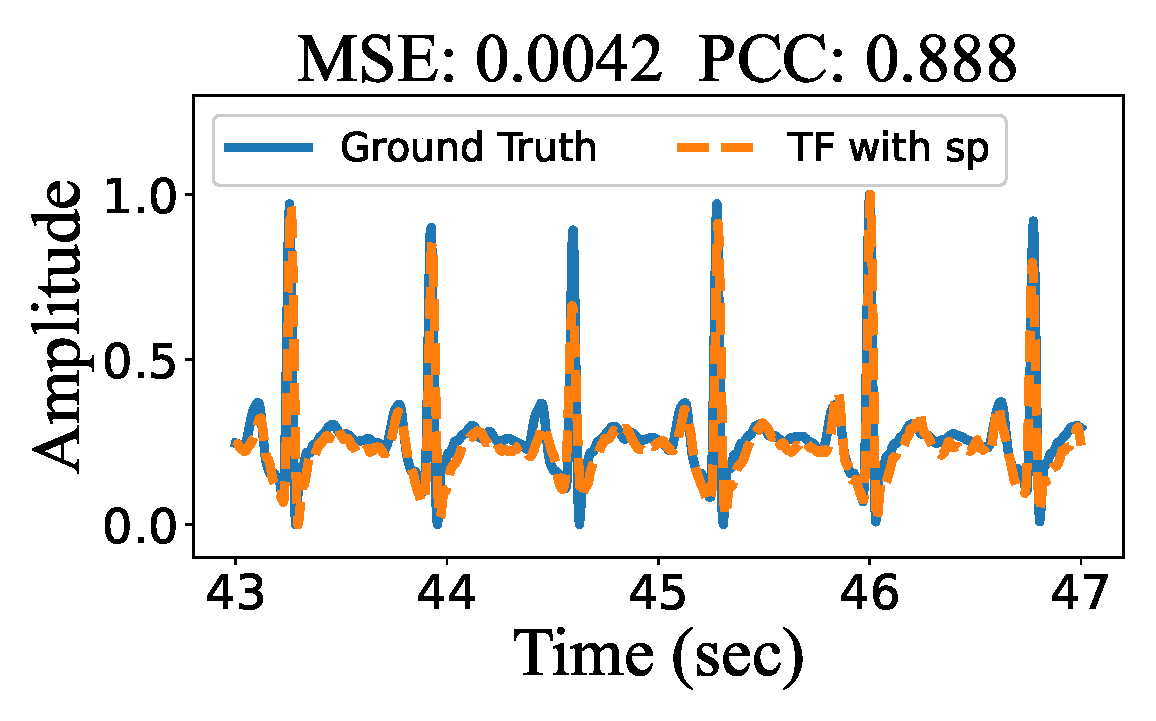
\includegraphics[width=0.4\columnwidth]{fs_good.eps}}
  \caption{Results of transfer learning using limited labeled data: (a) Poor ECG recovery without proper morphological feature and peak location; (b) Good ECG recovery owing to the pre-trained model.}
  \label{fig:fs_res}
\end{figure}


\begin{figure}[tb]
  \centering
  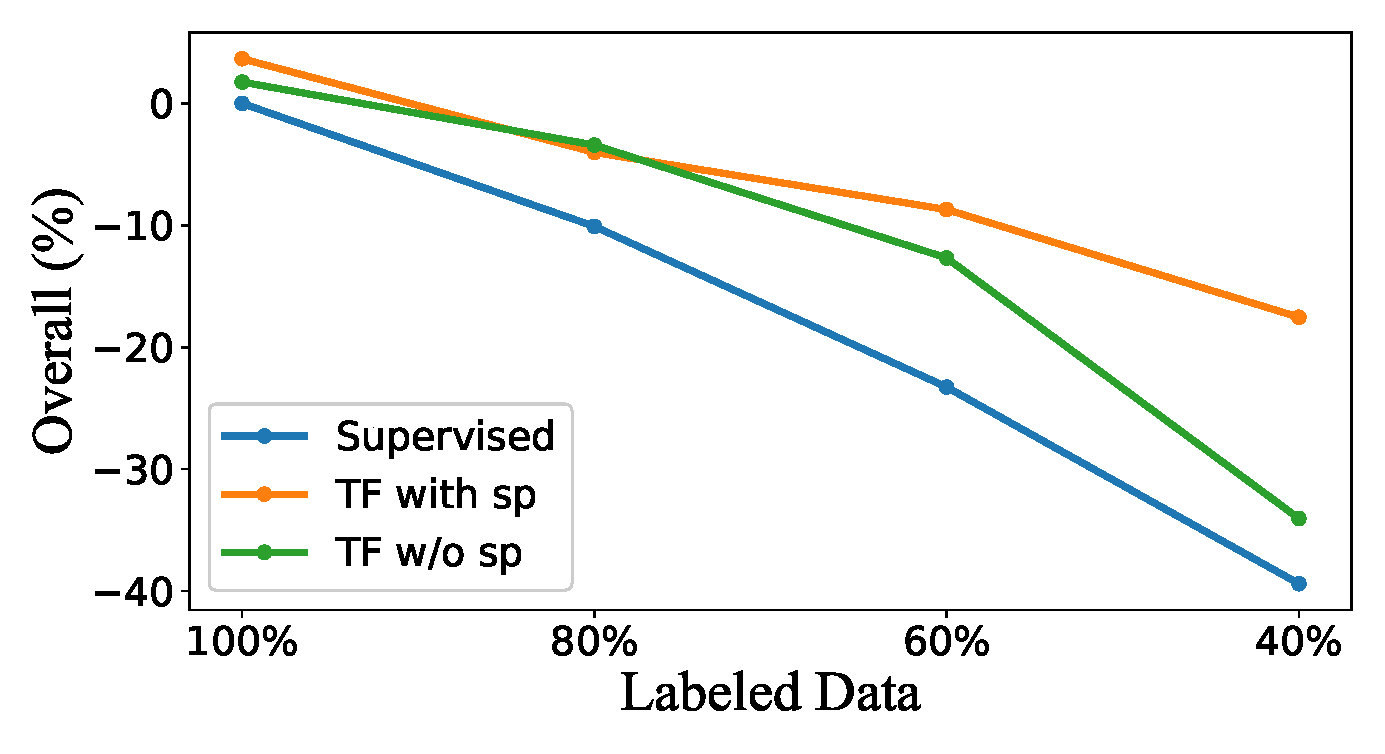
\includegraphics[width=0.7\columnwidth]{overall.eps}
  \caption{Overall performance of the radar-based ECG recovery.}
  \label{fig:overall}
\end{figure}
\subsection{Summary of Transfer-learning-based ECG Recovery}
Previous evaluations in terms of SSL and fine-tuning stages have illustrated the ability of the proposed RFcardi to learn from unlabeled data and transfer the knowledge to the ECG recovery task using limited radar-ECG pairs. The overall performance in Table~\ref{tab:ecg_few_shot} are plotted in Figure~\ref{fig:overall} for a straightforward comparison:
\begin{itemize}
  \item The performance of supervised learning drops heavily and cannot ensure high-quality ECG recovery after reducing $40\%$ labeled dataset.
  \item Transfer learning could enhance the performance of ECG recovery for the cases with ample labeled training data, and the quality of the pre-trained model has a minor effect on the final result because the deep learning model could learn from numerous radar-ECG pairs.
  \item For the cases with limited labeled data ($40\%$, $60\%$), the proposed RFcardi shows outstanding performance owing to the representations learned from unlabeled data. Furthermore, the quality of the pre-trained model does matter to alleviate the burden of deep learning model to learn both morphological ECG patterns and peak locations, as indicated by the increasing gap between orange and green lines in Figure~\ref{fig:overall}.
\end{itemize}

\section{Conclusion}\label{sec:conclusion_cp7}
This study proposes the data augmentation technique, Horcrux, for radar-based cardiac feature extraction with deep learning frameworks. Different from the traditional augmentation methods that may block the crucial parts or destroy the time consistency between input and ground truth, Horcrux preserves the percussive features of the input signal and only masks the cardiac-feature-related region on the harmonic spectrogram, enhancing the diversity of the limited dataset and also encouraging the deep learning model to only focus on the domain-preserved features. Compared with the existing methods, Horcrux reveals outstanding performance in heartbeat detection and ECG recovery and could effectively alleviate the degradation caused by the limited data. In addition, a transfer learning framework RFcardi is designed with SSR as a pre-text task for pre-training to reduce the dependency on cumbersome ECG ground truth collection. The experiments performed in different scenarios prove the feasibility of the CFT-RFcardi framework in radar signal extraction and ECG recovery with limited labeled data, enabling a convenient deployment in new scenarios with limited data for future contactless wellness monitoring.